\section{Related work}

\subsection{Classic software design approach}
Explain what it lacks

C does not do any run time or compile time bounds checking in arrays. At run time the code will just access or mangle whatever memory it happens to hit and crash or misbehave in some unpredictable way thereafter. "Professional programmer's language." - Nick Parlante\cite{clanguage}

\subsection{Other model based design approaches}
In 2014, another competing team has turned towards model based design [cite, Need for PID]. Blabla about their results.
Explain what it lacks. (special hardware requirements for example)

\subsection{Background} 

For the \textbf{RobonAUT 2014} contest, we used \verb!MATLAB! and \verb!Simulink! to implement the control system and the state machine. We chose the \verb!MathWorks! product family, because \verb!Simulink! has extensive support for model and simulation based development, and supports the generation of generic \verb!C! source code that can be later used on any hardware that is capable of running \verb!FreeRTOS! or any other hard real-time operating systems.

Figure \ref{fig:architecture} depicts the system architecture and stages of deployment. A typical system developed in \verb!MATLAB! can be divided to the following objects.

\begin{enumerate}
\item A \verb!MATLAB! \verb!Script! that defines the system model and computes the simulator and controller parameters.
\item Based on these parameters we can build the simulator and control software in \verb!Simulink! that interact with each other.
\item If the system response in the simulation is correct, the controller is ready for code generation, and field-testing.
\item The generated source code is invoked by the core operating system, the \verb!FreeRTOS! in this case
\item All communication with the hardware in implemented by the Core.
\end{enumerate}

\begin{figure}[!ht]
    \centering
    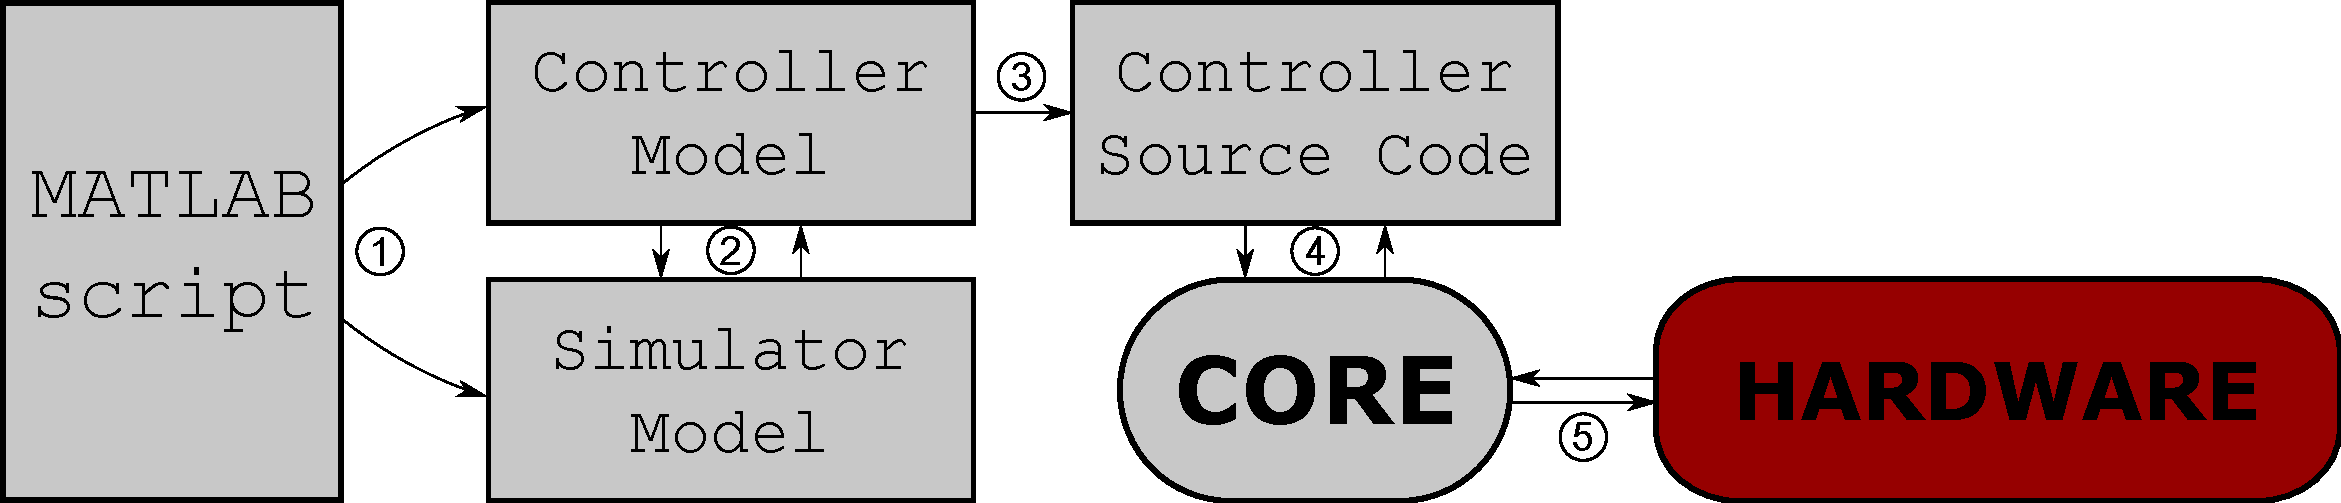
\includegraphics[width=\linewidth]{img/architecture}
    \caption{System architecture}
    \label{fig:architecture}
\end{figure}

% Contributions
\section{Model based design of the high level software}

As described earlier, the Model based design is based on solving the problems in a more visual environment. During the development, there's  limited connection between the designed software and the real hardware, as many of the solutions can be verified using the simulated model of the system.

In addition, with the use of the correct methods the result is not only the solution for the problem, but an automation that can formulate this solution for a given model. This means, that even if significant changes occur in the specifications, only minimal amount of modification is required to the code that formulates the software. This advantage can't be over emphasized, because the final specifications of the system are rarely known, especially in prototype development.

\subsection{Functional description}

During the race, the track is marked by a dark line on light ground. The car follows this line that guides it through certain checkpoints. Between checkpoints, there are obstacles that need to be passed in a specific way. Each obstacle is marked in a unique manner that allows the car to unambiguously determine, based on simple on-board sensors, which function it has to execute in the current segment.

The recommended sensor loadout\cite[sensors] is a number of optoelectronic sensors beneath the front axis or bumper of the car, and a couple of infrared proximity sensors to cover the front and the two sides of the car. Certain teams extended this setup with a camera for image-recognition, a second optosensor array and other methods. We sticked to the basic recommended sensor outfit, and this paper will not consider any other layouts.

\subsection{Building a model}

The first step in model based design is to create a model of the system, based on the functional description and known sensor loadout. To follow the line, the signals of the optical array must be processed and a control system must use this input to keep the car on the track. Let's define the following state variables:

\begin{center}
  \begin{tabular}{| c | p{0.8\linewidth} |}
\hline
    d & Position error: The shortest distance between the center of the front optical array and the center of the track \\ \hline
    $ \delta $ & Angular error: The angle between the centerline of the body and the tangent of the track \\ \hline
    $ \Phi $ & Steering angle: The effective steering angle, according to Ackermann-steering \\
    \hline
    $ \kappa $ & Current curvature of the track ($1/R$) \\ \hline
    x & Line position: the position of the track line along the front optical array \\ \hline
    c & Line speed: derivative of x, the change of the track line position \\ \hline
    v & Car speed: The current speed of the car along the centerline \\
    \hline
  \end{tabular}
\end{center}

Illustrating the system can help to visualize the relationships:

\begin{figure}[!ht]
    \centering
    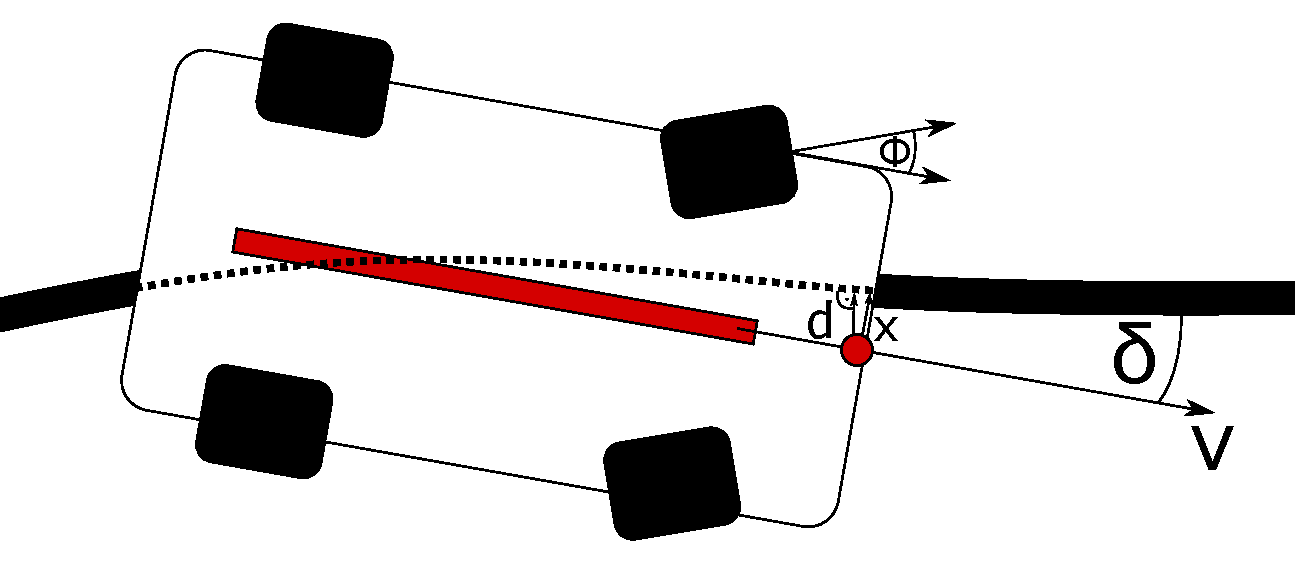
\includegraphics[width=\linewidth]{img/cartop}
    \caption{System model}
    \label{fig:cartop}
\end{figure}

\paragraph{Formulating the system model}

the first step is to implement the system descriptor script. In the following we'll build a steering controller.

Knowing the dynamical system equations~(\ref{eq:of1}, \ref{eq:of2}), and parameters (L: wheelbase), we can formulate the \textbf{A} (system transition) and \textbf{B} (system update) matrices linearly approximated in the equilibrium $(d = 0; \delta = 0; v = 1)$ ~(\ref{eq:of3}).

\begin{align} 
    \dot{d} &= sin(\delta + \Phi) \cdot v  \label{eq:of1} \\ 
    \dot{\delta} &= \frac{v}{L} \cdot tan(\Phi) + \kappa \label{eq:of2}
\end{align}

% \begin{minipage}{0.45\linewidth}
%     \begin{align} \label{eq:of3}
%         \begin{bmatrix}
%                \dot{d} \\
%                \dot{\delta}
%         \end{bmatrix}
%         =
%         \begin{bmatrix}
%                0 & \delta \cdot v \\
%                0 & 0
%         \end{bmatrix}
%         %\cdot
%         \begin{bmatrix}
%                d \\
%                \delta
%         \end{bmatrix}
%      \end{align}
% \end{minipage}
% \begin{minipage}{0.45\linewidth}
%     \begin{align} \label{eq:of4}
%         \begin{bmatrix}
%                \dot{d} \\
%                \dot{\delta}
%         \end{bmatrix}
%         =
%         \begin{bmatrix}
%            0 & 0 \\
%            \frac{v}{L} & 1
%          \end{bmatrix}
%         %\cdot
%          \begin{bmatrix}
%                \Phi \\
%                \kappa
%         \end{bmatrix}
%      \end{align}
% \end{minipage}

    \begin{align} \label{eq:of3}
        \begin{bmatrix}
               \dot{d} \\
               \dot{\delta}
        \end{bmatrix}
        =
        \begin{bmatrix}
               0 & \delta \cdot v \\
               0 & 0
        \end{bmatrix}
        %\cdot
        \begin{bmatrix}
               d \\
               \delta
        \end{bmatrix}
		+
        \begin{bmatrix}
           0 & 0 \\
           \frac{v}{L} & 1
         \end{bmatrix}
        %\cdot
         \begin{bmatrix}
               \Phi \\
               \kappa
        \end{bmatrix}
     \end{align}

Instead of hard-coding the system matrices into the script, we can apply a different method that is closer to the model based approach, by using the \verb!MATLAB! \verb!Symbolic! \verb!Toolbox!. This package allows the automatic generation of the Jacobi-matrices of the system, so the inputs are narrowed down to the system parameters and nonlinear dynamic equations. Furthermore, this way we can hold on to a lot more information that can later be used to generate a nonlinear state observer, Extended Kalman Filter[appendix?], or Hybrid Linear Controller[appendix?].

[figure: partial prev figure extended with an above-top symbolic layer]
     
\begin{minipage}{0.45\linewidth}
    \begin{align}
        A_J =
        \begin{bmatrix}
           \frac{\partial \dot{d}}{\partial d} & \frac{\partial \dot{d}}{\partial \delta} \\
           & \\
           \frac{\partial \dot{\delta}}{\partial d} & \frac{\partial \dot{\delta}}{\partial \delta}
         \end{bmatrix}
     \end{align}
\end{minipage}
\begin{minipage}{0.45\linewidth}
    \begin{align}
        B_J =
         \begin{bmatrix}
               \frac{\partial \dot{d}}{\partial \Phi} \\
               \\
               \frac{\partial \dot{\delta}}{\partial \Phi}
        \end{bmatrix}
     \end{align}
\end{minipage}

\begin{lstlisting}
    % Definition of system equations
    d_dot = sin(Delta + Phi) * v;
    Delta_dot = v/L * tan(Phi) + Kappa;
    
    % Computing the Jacobi matrices
    A_sym = [0      diff(d_dot, Delta);
             0      0                ];
       
    B_sym = [diff(d_dot, Phi);
             diff(Delta_dot, Phi)];
    
    % Substitution of approximation points
    A = double(subs(A_sym, [L, d, Delta, Phi, v],...
        [L_car, 0, 0, 0, 1]));
    B = double(subs(B_sym, [L, d, Delta, Phi, v],...
        [L_car, 0, 0, 0, 1]));
\end{lstlisting}

\paragraph{Control system}

Once an accurate system model is available, it's possible to formulate a controller. It's relatively easy to implement multiple controllers and compare their effectiveness on the simulated system to determine, which would fit the robot the best.
Already knowing the state-space form of the system, a full-state feedback controller can be formulated quickly to stabilize the system. Using the Ackermann formula, we get the feedback matrix.

\begin{lstlisting}
    % Definition of remaining state-space matrices
    C = [1 0];
    D = 0;
    sys = ss(A,B,C,D);
    
    % Controller design
    P = [-3 -3];
    K = acker(A,B,P);
    sys_c = ss(A-B*K, B, C, D);
\end{lstlisting}

If we check the results we can see that the system has been stabilized.

\begin{figure}[!ht]
    \centering
    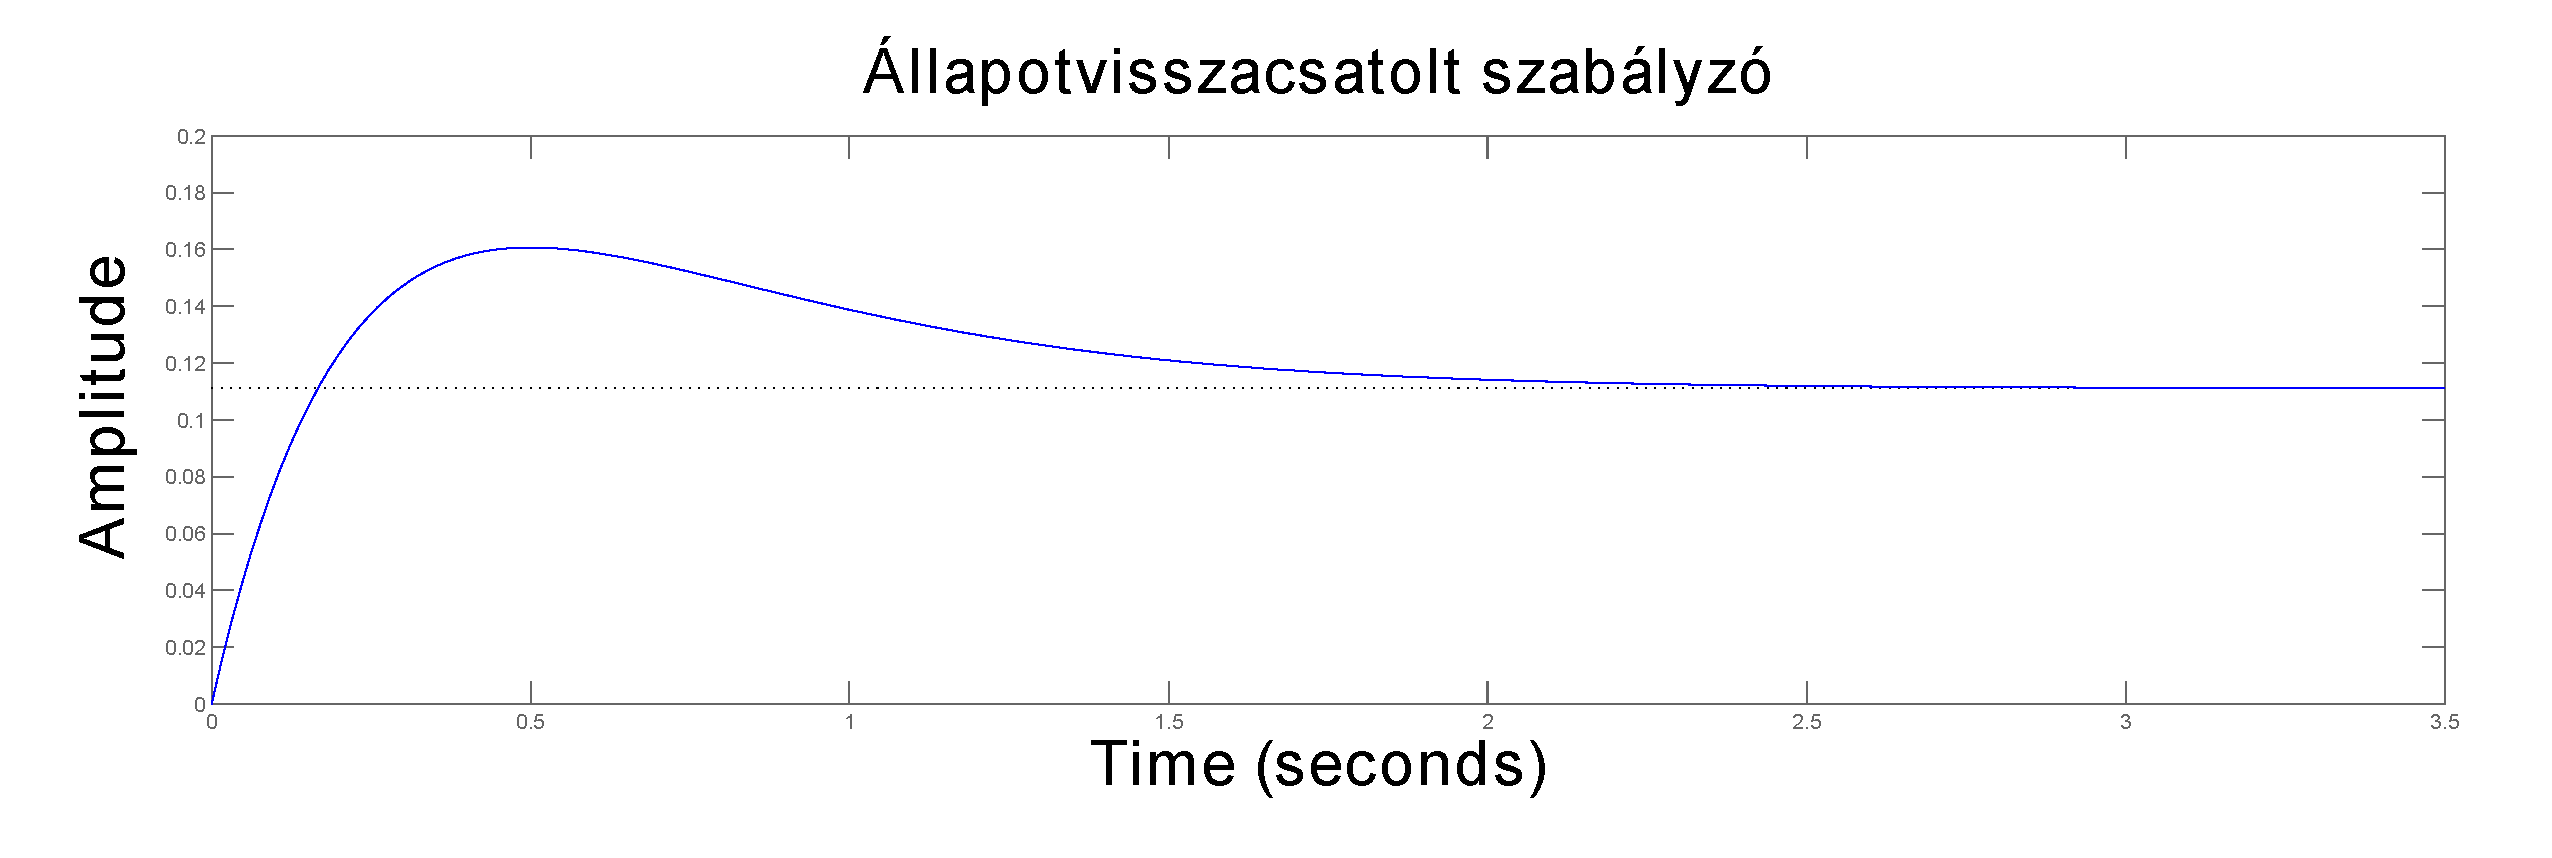
\includegraphics[width=\linewidth]{img/plot2}
    \caption{Instabil rendszer állapotvisszacsatolt stabilizációja}
    \label{fig:plot2}
\end{figure}

\paragraph{Direct and inverse measurement models}

Unfortunately, a full-state feedback loop can rarely be realized directly, and the controller we have just created would not be able to control the actual system. Certain states can not be observed directly, and can only be estimated by a state observer. Simulating the sensor readings based on the state variables can be done with the \emph{Direct measurement model}, while in order to estimate the states based on the sensor reading we need the \emph{inverse measurement model}.

Knowing the geometrical layout of the car, the expected sensor readings can be simulated using geometrical projection to the optosensor array:

\begin{align}
    x = \frac{d}{\cos(\delta)}
\end{align}

After the direct model has been determined, the inverse model can be formulated as well:

\begin{align}
    \hat{d} &= x \cdot \cos(\delta) \\
    \hat{c} &=\dot{x} \\
    \hat{\delta} &= \arctan \left(\frac{c}{v}\right) - \Phi
\end{align}

The direct model is usually part of the simulation only, however it's possible to proof-check the sensor readings during run-time. This can be especially useful, if we plan to produce the estimated states using sensorfusion. The inverse measurement model is always the first layer of the control loop, while it is rarely found in the simulated environment.

Note: $\delta$ can be directly measured if the robot is equipped with multiple optosensor arrays.

\subsection{Building the simulation environment}

When a sufficient model and controller are available, it is time to build the simulation environment. In case of a simple system, at this point the controller could be implemented directly in \verb!C!, but in case of a complex system it is better practice to go through with the model based design.



A rendszert két fő logikai részre bonthatjuk, az \textbf{Irányító rendszerre} és a \textbf{Szimulátorra}, illetve egy harmadik blokk interfészt biztosít e kettő között. A MATLAB (így a Simulink is) gyengén típusos nyelv, de lehetőség van a típusok erős állítására is. Ez beágyazott rendszereknél különösen hasznos, mivel a MATLAB egészen meglepő típusokat tud előállítani magának, ami nem előnyös sem a futási sebesség, sem a kézbentarthatóság szempontjából, különösen ha fixpontos számábrázolással szeretnénk dolgozni.

\paragraph{Szimulátor}

A megállapított rendszermodell alapján felépíthetjük a szimulátort. Hiába terveztük a szabályzót a linearizált modellhez, a szimulátornak mindig a legelső lépésben meghatározott, gyakran nemlineáris összefüggések alapján kell felépülnie, különben csak magunkat csapjuk be a hibás szimulációval, és az egész technológia nem ér semmit.
A nemlineáris rendszerek felépítéséhez kiváló segédletet nyújt a Szabályozástechnika tárgy 5-6. gyakorlata, illetve annak felkészülési anyaga\cite[p.~319-354]{szabtech}, így erre nem térünk ki. Amennyiben a rendszermodellt a Jacobi mátrixok segítségével generáltuk, célszerűbb közvetlenül azt felhasználni a szimulációban a blokkokból felépített rendszer helyett, így nem csak paraméter-, hanem rendszerszintű változás esetén sem kell kézzel utólag módosítani a szimulátort.

\begin{figure}[!ht]
    \centering
    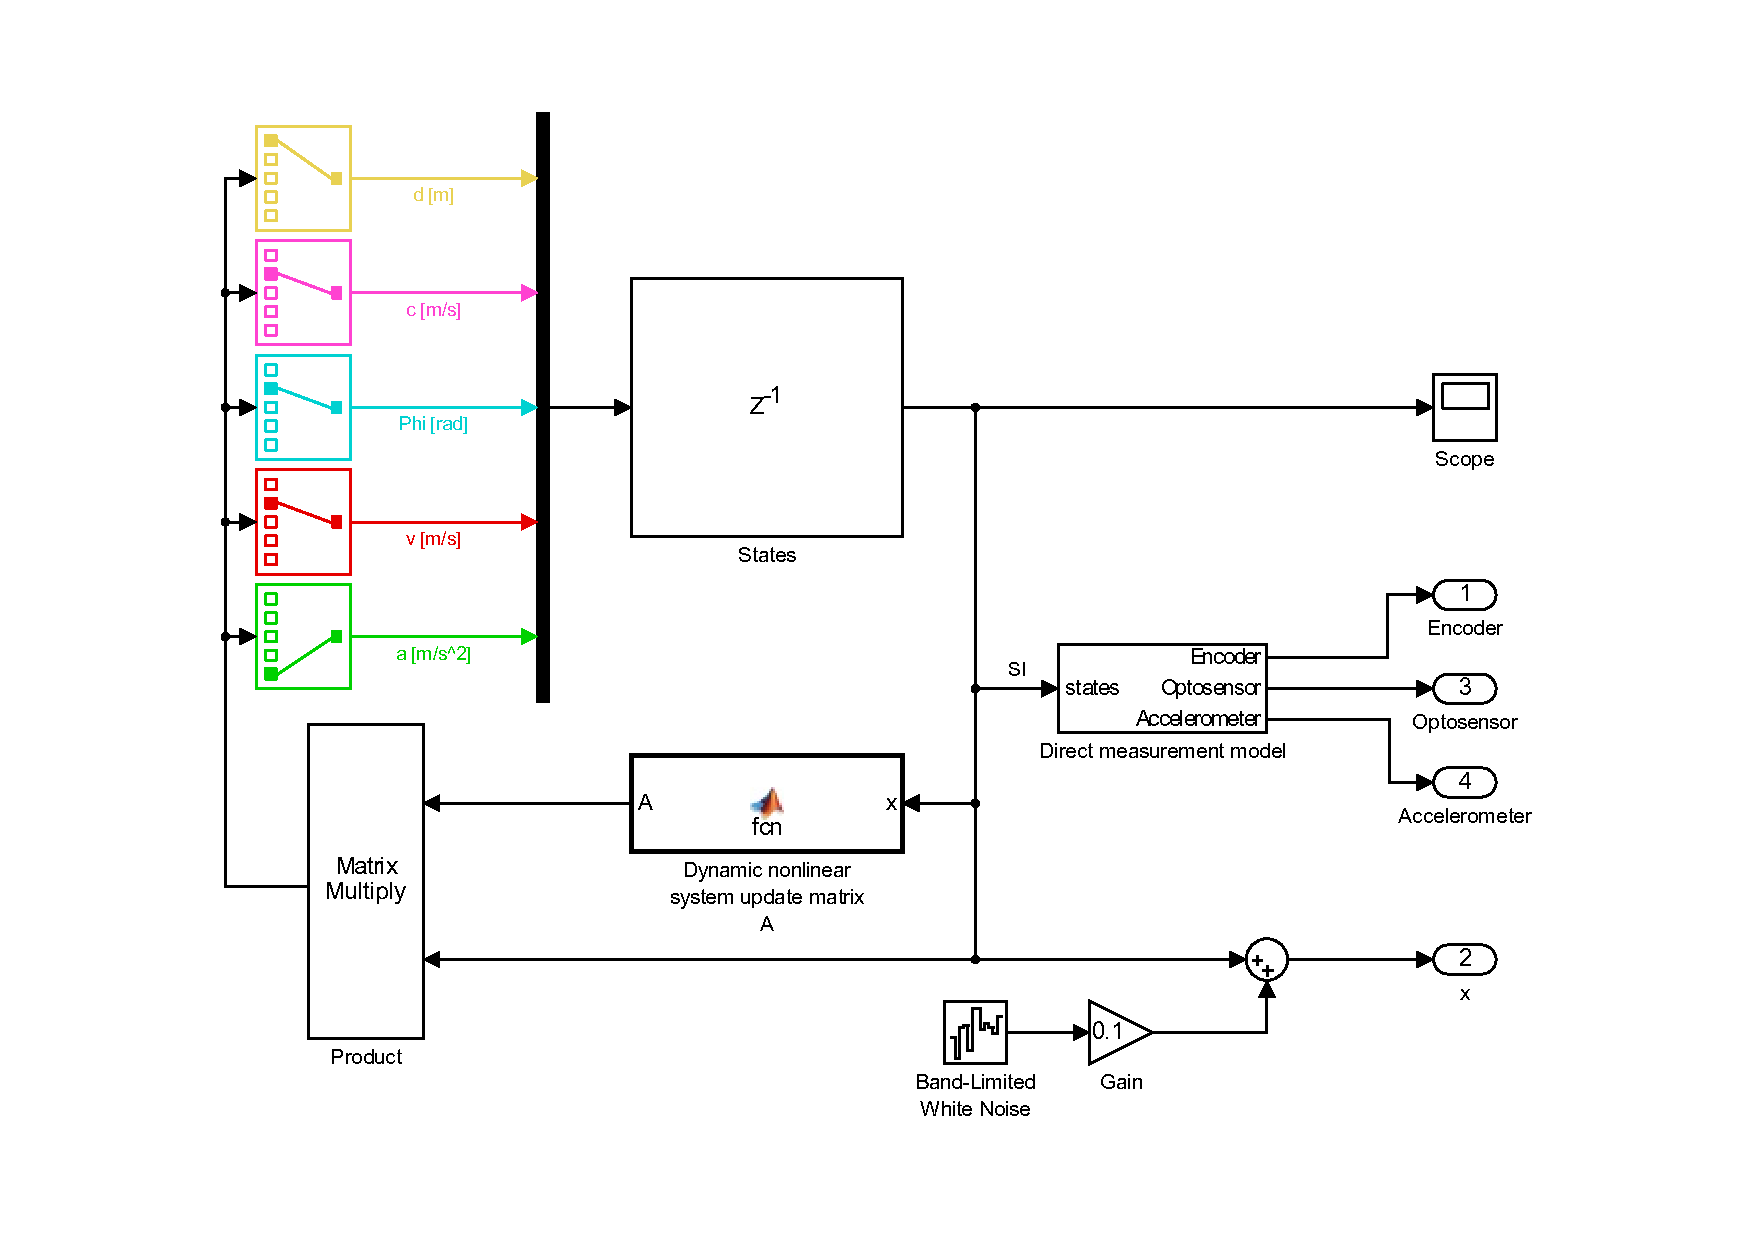
\includegraphics[width=\linewidth]{img/sys}
    \centering
    \vspace{-30pt}
    \caption{Jacobi-mátrix alapú nemlineáris szimulátor blokkdiagram}
    \label{fig:model}
\end{figure}

Ne feledjük, a szimulátor kimenete nem csupán az állapot, hanem a direkt mérési modell által előállított szimulált szenzorjelek, melyeket mesterségesen zajjal is terhelhetünk, hogy eggyel kevesebb meglepetés érjen a tényleges teszteléskor.

\subsection{Implementation of a complex control system}

Az irányítás tetszőlegesen bonyolult lehet, a RobonAUT-hoz készült megoldás 4 fő kritikus (működéshez elengedhetetlen) részre bontható:

\paragraph{Inverz mérési modell}

A korábban vázolt inverz mérési modell megvalósítása, célja a \textbf{visszacsatolt, mérhető állapotok} előállítása a szenzorok jelei alapján, tehát \textbf{priori információk nélkül}. Mivel a verseny során többféle jelre kellett szabályozni (vonaldetektálás, bal/jobb éldetektálás, bal/jobb távolságérzékelő szenzor jele), ezekre mind létre kell hozni az inverz mérési modellt, majd a megfelelő visszacsatolt állapotot adni tovább a jelfeldolgozónak.

\paragraph{Jelfeldolgozó és állapotbecslő}

Az inverz mérési modell által előállított \textbf{visszacsatolt állapotokat} dolgozza fel \textbf{priori információk} segítségével. Ez a mi esetünkben egy Kálmán-szűrőt jelentett, ahol a mérési jel a visszacsatolt állapot, a priori információ pedig a rendszer modellje. Bár a Kálmán-szűrő támogatja az inverz mérési modell közvetlen integrálását a szűrőbe, ezt a megoldást nem találtam célszerűnek, mivel a szenzorsor jelvektorából a vonal pozíciójele nem állítható elő zárt mátrixos alakban, valamint többféle jelentősen eltérő lehetséges bemenet között kell kapcsolni.

\paragraph{Szabályzó}

A szabályzó a szkript alapján számított paraméterek alapján implementálható, ez függ a választott szabályzó típusától és a tervezés módjától.

\paragraph{Magas szintű irányítás, állapotgép}

A magas szintű irányítás felel a szabályzás és állapotgép alapján történő vezérlés közötti kapcsolásért és a szabályzó bemeneti jelének kiválasztásáért, az aktuális állapot szerint. Ezenkívül referenciajeleket határozhat meg a sebességnek és a kormányszabályzónak.

\subsection{Preparing MATLAB Coder for code generation}

Az elkészült szabályzóból \verb!C! (vagy \verb!C++!, \verb!Verilog! és \verb!PLC!) kódot generálhatunk, melyet beágyazhatunk a rendszerbe. A generált kód egyfajta statikus osztályként működik, vannak belső tárolói és tagfüggvényei, de nem szükséges a példányosítása.

Az első lépés a kódgenerálás előkészítéséhez a megfelelő \textbf{solver} beálítása. Ezt a \textbf{Simulation/Configuration parameters... (Ctrl + E)} menüpontban tehetjük meg a \textbf{Solver} menüpontban. A típust Fixed-step-re kell állítani, a solvert pedig discrete-re, hogy ne legyenek folytonos állapotok a modellünkben. Ezután ne felejtsük el megadni a mintavételi idejét a rendszernek, másodpercben.
Ezt a beállítást célszerű már a modell létrehozásakor, a legelső lépésként elvégezni, ugyanis egy folytonos környezetben épített modell nem feltétlenül fog működni diszkrét solverrel! (Alternatív módon \textbf{Atomic Subsystem} blokkba helyezhetjük a fordítani kívánt rendszert, amennyiben mindenképpen folytonos idejű szimulátorral szeretnénk dolgozni. Ekkor nem szükséges a solver módosítása, viszont gondoskodni kell a mintavételi idő váltásról.)

A tényleges kódgeneráláshoz szükség van egy MATLAB által támogatott \verb!C/C++! compilerre is. A teljes lista megtekinthető a MathWorks weboldalán.\footnote{http://www.mathworks.com/support/compilers/}

\paragraph{Target beállítása}

A kódgenerálásra millióféle különböző beállítás létezik, ezek közül az STM32F4-Discovery kártyához tartozót mutatjuk be, mivel ez volt a célplatform a RobonAUT verseny során.

A \textbf{Hardware Implementation} menüpontban a \textbf{Device Vendor} legördülő listát állítsuk \textbf{ARM Compatible}-re, a \textbf{Device type}-ot pedig \textbf{ARM Cortex}-re.
A \textbf{Code Generation} menüpontban állítsuk át a \textbf{System target file}-t \textbf{ert.tlc}-re (ezzel az általános MATLAB-Embedded codert hívjuk meg).
Az \textbf{Interface} menüpontban a \textbf{Code Replacement Library}-t állítsuk \textbf{GCC ARM Cortex-M3}-re.
Amennyiben lebegőpontos számábrázolást is használunk a programban, kapcsoljuk be ezeknek a támogatását. Kihasználatlanul viszont nem javasolt mindent bekapcsolni, mivel csak felesleges típusdefiníciók jönnek létre. Ha valamit elfelejtettünk beállítani, Build közben hibajelzéssel ide fog visszairányítani a MATLAB.
A \textbf{Report} menüpontban bekapcsolható a "Create code generation report", ami egy dokumentációt is generál a kód mellé.
A \textbf{Code Generation} menüponthoz visszatérve bekapcsolhatjuk az optimalizációkat is, így javíthatunk a kód futásteljesítményén, valamint a generálás sebességén növelhetjük, ha nem kérünk make-filet, illetve buildet egyből, hanem csak a kódot állítjuk elő (úgyis csak arra van szükségünk itt).
A kezelhetőséget javítja, ha a \textbf{Code placement}-ben a \textbf{Code packaging}-et \textbf{Compact}-ra állítjuk, így kevesebb forrásfájlt generál, és könnyebb kezelni, ha csak egy generált rendszerünk van.

\paragraph{Tl;dr}

\begin{itemize}

    \item \textbf{Solver} $\rightarrow$ Fixed step, discrete
    \item \textbf{Hardware Implementation} $\rightarrow$ Device type $\rightarrow$ ARM Cortex
    \item \textbf{Code Generation} $\rightarrow$ System Target File $\rightarrow$ ert.tlc
    \item \textbf{Interface} $\rightarrow$ Code Replacement Library $\rightarrow$ GCC ARM Cortex-M3
    \item \textbf{MATLAB Command Line} $\rightarrow$ \textbf{mex -setup}

\end{itemize}

A megfelelő beállítás után a Simulink modellben keressük meg azt a blokkot, melyből kódot szeretnénk generálni. Egy nagy rendszerben akár több részben is lehet kódot generálni, pl. kapcsolható működés, vagy eltérő mintavételi idő esetén hasznos. Jelen esetben az Irányító rendszer blokkját szeretnénk felhasználni, melynek bemenete a szenzoroktól kapott közvetlen jel, kimenete pedig a szervójel. A blokkon jobb kattintás, majd \textbf{C/C++ Code} $\rightarrow$ \textbf{Build This Subsystem} (Régebbi MATLAB verziókban MATLAB Coder, illetve Real Time Workshop (RTW) menüpontokat kell keresni). A generált fileok a \verb!MATLAB Current Working Folder!-be kerülnek, nem a modell mappájába.









